\section{eo\-VRPGeneric\-Crossover Class Reference}
\label{classeo_v_r_p_generic_crossover}\index{eoVRPGenericCrossover@{eoVRPGenericCrossover}}
Implementation of the generic crossover for the VRP-TW by Tavares et al.  


{\tt \#include $<$eo\-VRPQuad\-Crossover.h$>$}

Inheritance diagram for eo\-VRPGeneric\-Crossover::\begin{figure}[H]
\begin{center}
\leavevmode
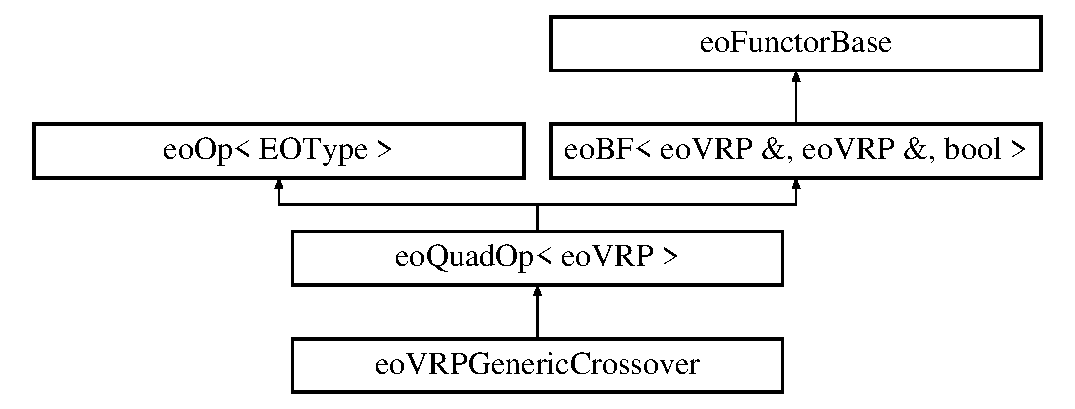
\includegraphics[height=4cm]{classeo_v_r_p_generic_crossover}
\end{center}
\end{figure}
\subsection*{Public Member Functions}
\begin{CompactItemize}
\item 
\bf{eo\-VRPGeneric\-Crossover} ()\label{classeo_v_r_p_generic_crossover_63e5fb734c46be62a12f6799e34cebe4}

\begin{CompactList}\small\item\em Deafult constructor. \item\end{CompactList}\item 
std::string \bf{class\-Name} () const 
\begin{CompactList}\small\item\em Returns a string containing the name of the class. \item\end{CompactList}\item 
bool \bf{operator()} (\bf{eo\-VRP} \&\_\-genotype1, \bf{eo\-VRP} \&\_\-genotype2)
\begin{CompactList}\small\item\em Both parameters are the parents and the (future) children of the crossover. \item\end{CompactList}\end{CompactItemize}
\subsection*{Private Member Functions}
\begin{CompactItemize}
\item 
bool \bf{Generic\-Crossover} (const Routes \&\_\-donor, Routes \&\_\-receiver) const 
\begin{CompactList}\small\item\em Actually performs the generic crossover. \item\end{CompactList}\end{CompactItemize}


\subsection{Detailed Description}
Implementation of the generic crossover for the VRP-TW by Tavares et al. 



Definition at line 53 of file eo\-VRPQuad\-Crossover.h.

\subsection{Member Function Documentation}
\index{eoVRPGenericCrossover@{eo\-VRPGeneric\-Crossover}!className@{className}}
\index{className@{className}!eoVRPGenericCrossover@{eo\-VRPGeneric\-Crossover}}
\subsubsection{\setlength{\rightskip}{0pt plus 5cm}std::string eo\-VRPGeneric\-Crossover::class\-Name (void) const\hspace{0.3cm}{\tt  [inline, virtual]}}\label{classeo_v_r_p_generic_crossover_7740db73b7151dab52df9d50f5366429}


Returns a string containing the name of the class. 

Used to display statistics. \begin{Desc}
\item[Returns:]The string containing the name of the class. \end{Desc}


Reimplemented from \bf{eo\-Quad\-Op$<$ eo\-VRP $>$}.

Definition at line 71 of file eo\-VRPQuad\-Crossover.h.\index{eoVRPGenericCrossover@{eo\-VRPGeneric\-Crossover}!operator()@{operator()}}
\index{operator()@{operator()}!eoVRPGenericCrossover@{eo\-VRPGeneric\-Crossover}}
\subsubsection{\setlength{\rightskip}{0pt plus 5cm}bool eo\-VRPGeneric\-Crossover::operator() (\bf{eo\-VRP} \& {\em \_\-genotype1}, \bf{eo\-VRP} \& {\em \_\-genotype2})\hspace{0.3cm}{\tt  [inline, virtual]}}\label{classeo_v_r_p_generic_crossover_d7d3b19562b071bd50dd4d831e447d0c}


Both parameters are the parents and the (future) children of the crossover. 

\begin{Desc}
\item[Parameters:]
\begin{description}
\item[{\em \_\-genotype1}]The first parent. \item[{\em \_\-genotype2}]The second parent. \end{description}
\end{Desc}
\begin{Desc}
\item[Returns:]True if any of the parents was modified. False otherwise. \end{Desc}


Implements \bf{eo\-BF$<$ eo\-VRP \&, eo\-VRP \&, bool $>$}.

Definition at line 85 of file eo\-VRPQuad\-Crossover.h.

References eo\-VRP::encode(), Generic\-Crossover(), and eo\-VRP::routes().\index{eoVRPGenericCrossover@{eo\-VRPGeneric\-Crossover}!GenericCrossover@{GenericCrossover}}
\index{GenericCrossover@{GenericCrossover}!eoVRPGenericCrossover@{eo\-VRPGeneric\-Crossover}}
\subsubsection{\setlength{\rightskip}{0pt plus 5cm}bool eo\-VRPGeneric\-Crossover::Generic\-Crossover (const Routes \& {\em \_\-donor}, Routes \& {\em \_\-receiver}) const\hspace{0.3cm}{\tt  [inline, private]}}\label{classeo_v_r_p_generic_crossover_543ba6869b93a3f9f709045b7e24d74a}


Actually performs the generic crossover. 

\begin{Desc}
\item[Parameters:]
\begin{description}
\item[{\em \_\-donor}]Set of routes from the first parent. \item[{\em \_\-receiver}]Set of routes from the second parent \end{description}
\end{Desc}
\begin{Desc}
\item[Returns:]True if the second parent was modified. False otherwise. \end{Desc}


Definition at line 110 of file eo\-VRPQuad\-Crossover.h.

References eo\-Rng::random().

Referenced by operator()().

The documentation for this class was generated from the following file:\begin{CompactItemize}
\item 
eo\-VRPQuad\-Crossover.h\end{CompactItemize}
